%%%%%%%%%%%%%%%%%%%%%%%%%%%%%%%%%%%%%%%%%%%%%%%%%%%%%%%%%%%%%%%%%%%%%%%%
%                                                                      %
%     File: Thesis_Appendix_B.tex                                      %
%     Tex Master: Thesis.tex                                           %
%                                                                      %
%     Author: Andre C. Marta                                           %
%     Last modified :  2 Jul 2015                                      %
%                                                                      %
%%%%%%%%%%%%%%%%%%%%%%%%%%%%%%%%%%%%%%%%%%%%%%%%%%%%%%%%%%%%%%%%%%%%%%%%

\chapter{Option Market Data}
\label{chapter:mktdata}

Here, we present data for European options. For data compliance reasons, the strike prices were normalized by the initial stock price i.e. $K\rightarrow K/S_0$ so that the original strike prices are inaccessible.
Suffice it to say that the underlying asset of the options here represented is a \emph{stock index}, i.e. a weighted average of the prices of some selected stocks (e.g. PSI-20 (Portugal)).

The data provided pertains to the options' implied volatilities. We can easily obtain their prices from these values using eq.\eqref{impvolform}. The converted prices of call European options are shown below.

The number of days here denoted correspond to trading days (i.e. days where exchanges are open and trading occurs) so that one month corresponds to 21 days and one year to 252.

\begin{table}[!htb]
  \begin{adjustwidth}{-0.25cm}{-0.25cm}
  \begin{subfigmatrix}{2}
\subfigure{
\centering
\renewcommand{\arraystretch}{1.1}
\begin{tabular}{@{}cccc@{}}
\toprule
$T$(days) & $K$($\EUR$) & $\sigma_{imp,\mathrm{mkt}}$($\SI{}{\year\tothe{-0.5}}$) & $C_{\mathrm{mkt}}$($\EUR$) \\ \midrule
\multirow{7}{*}{21} & 0.50 & 0.7082 & \num{5.000E-01} \\
 & 0.75 & 0.4632 & \num{2.506E-01} \\
 & 0.90 & 0.2989 & \num{1.044E-01} \\
 & 1.00 & 0.2425 & \num{2.792E-02} \\
 & 1.10 & 0.2314 & \num{2.421E-03} \\
 & 1.25 & 0.2699 & \num{5.345E-05} \\
 & 1.50 & 0.3433 & \num{5.748E-07} \\ \midrule
\multirow{7}{*}{42} & 0.50 & 0.5556 & \num{5.000E-01} \\
 & 0.75 & 0.3876 & \num{2.519E-01} \\
 & 0.90 & 0.2824 & \num{1.107E-01} \\
 & 1.00 & 0.2461 & \num{4.006E-02} \\
 & 1.10 & 0.2354 & \num{8.525E-03} \\
 & 1.25 & 0.2525 & \num{6.209E-04} \\
 & 1.50 & 0.2968 & \num{1.583E-05} \\ \bottomrule
\end{tabular}}
\subfigure{
\centering
\renewcommand{\arraystretch}{1.1}
\begin{tabular}{@{}cccc@{}}
\toprule
$T$(days) & $K$($\EUR$) & $\sigma_{imp,\mathrm{mkt}}$($\SI{}{\year\tothe{-0.5}}$) & $C_{\mathrm{mkt}}$($\EUR$) \\ \midrule
\multirow{7}{*}{63} & 0.50 & 0.4789 & \num{5.001E-01} \\
 & 0.75 & 0.3452 & \num{2.530E-01} \\
 & 0.90 & 0.2658 & \num{1.153E-01} \\
 & 1.00 & 0.2401 & \num{4.787E-02} \\
 & 1.10 & 0.2330 & \num{1.421E-02} \\
 & 1.25 & 0.2438 & \num{1.799E-03} \\
 & 1.50 & 0.2749 & \num{7.656E-05} \\ \midrule
\multirow{7}{*}{126} & 0.50 & 0.3878 & \num{5.004E-01} \\
 & 0.75 & 0.2954 & \num{2.569E-01} \\
 & 0.90 & 0.2444 & \num{1.272E-01} \\
 & 1.00 & 0.2295 & \num{6.467E-02} \\
 & 1.10 & 0.2269 & \num{2.862E-02} \\
 & 1.25 & 0.2340 & \num{7.569E-03} \\
 & 1.50 & 0.2521 & \num{8.580E-04} \\ \bottomrule
\end{tabular}
}
  \end{subfigmatrix}
  \caption[Data to be used in model calibration and validation.]{Data to be used in model calibration and validation.}
  \label{tab:mktdata}
  \end{adjustwidth}
\end{table}



\begin{figure}[!htb]
  \begin{subfigmatrix}{2}
    \subfigure[Implied Volatility, T=21 days]{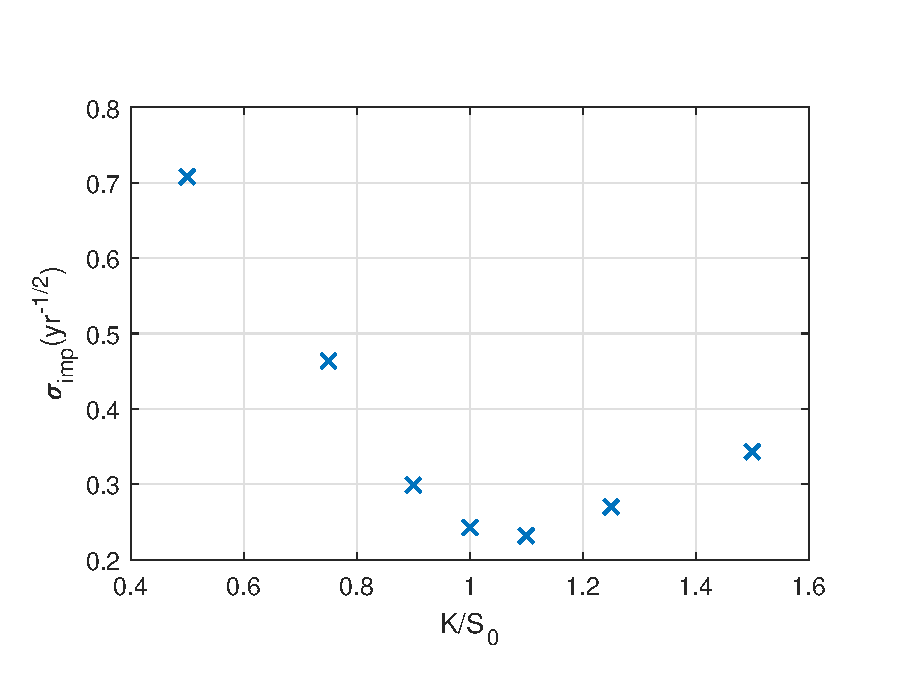
\includegraphics[width=0.47\linewidth,trim={0.25cm 0.45cm 1.1cm 1.4cm},clip]{T1.eps}}
    \subfigure[European Call Price, T=21 days]{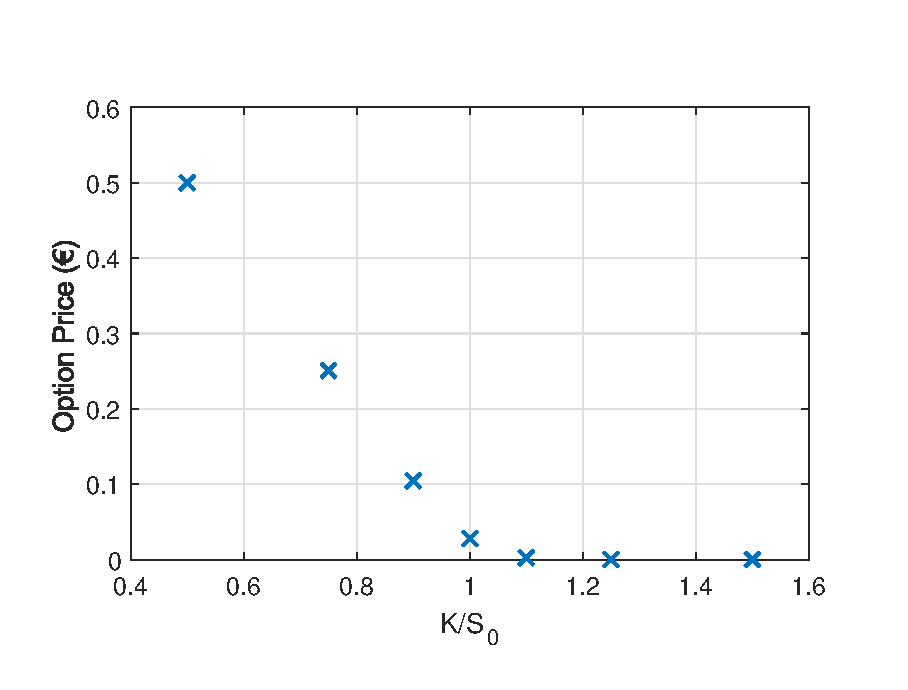
\includegraphics[width=0.47\linewidth,trim={0.25cm 0.45cm 1.1cm 1.4cm},clip]{T1P.eps}}
    \subfigure[Implied Volatility, T=42 days]{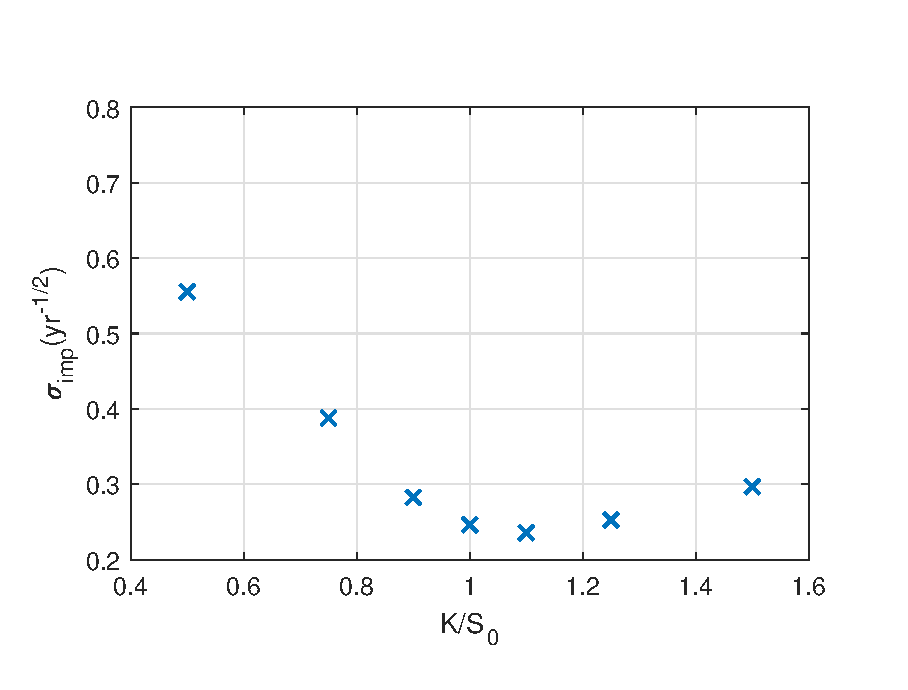
\includegraphics[width=0.47\linewidth,trim={0.25cm 0.45cm 1.1cm 1.4cm},clip]{T2.eps}}
    \subfigure[European Call Price, T=42 days]{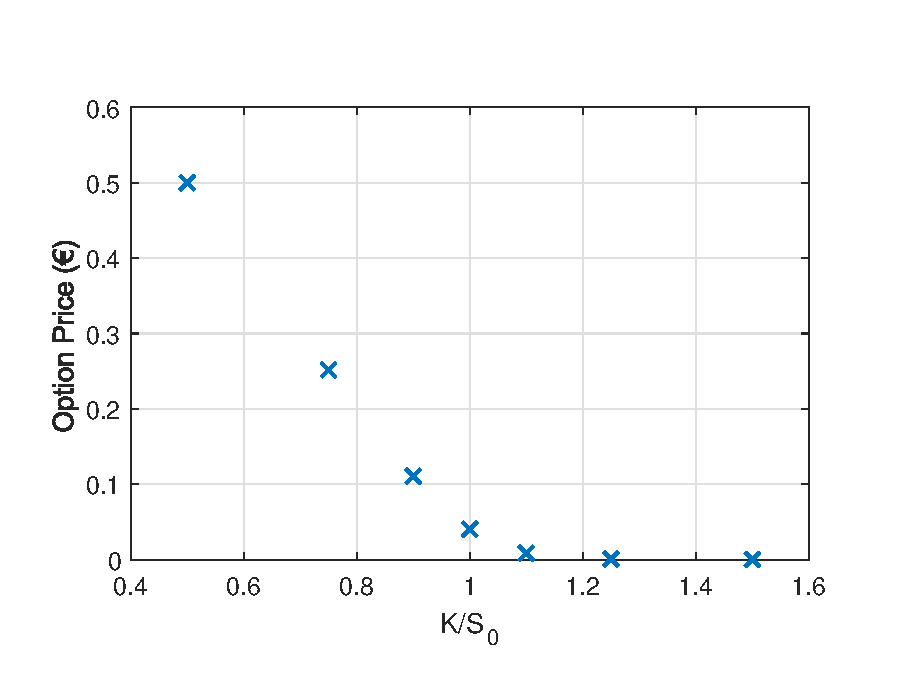
\includegraphics[width=0.47\linewidth,trim={0.25cm 0.45cm 1.1cm 1.4cm},clip]{T2P.eps}}
    \subfigure[Implied Volatility, T=63 days]{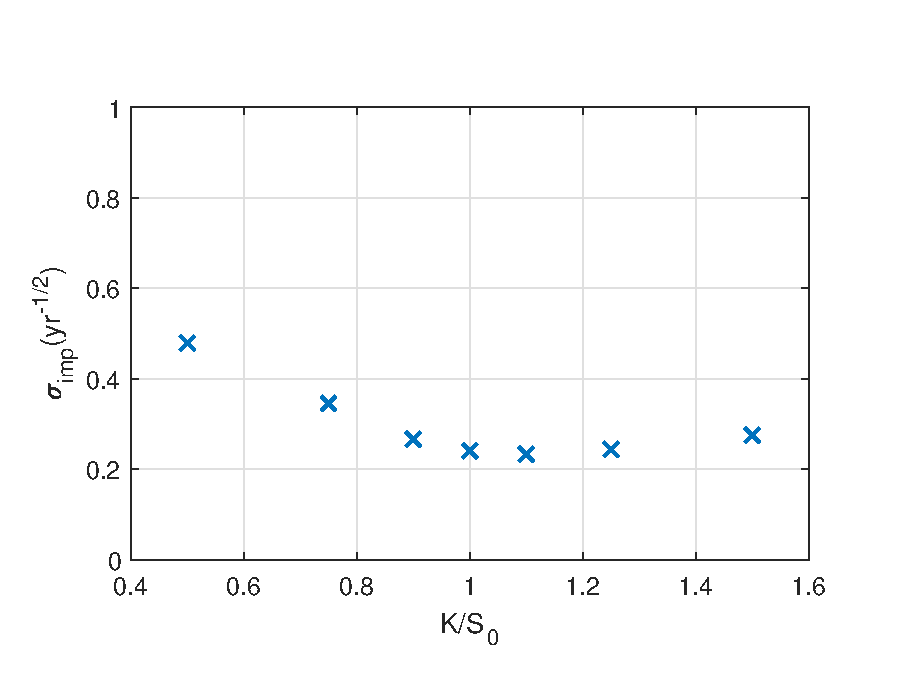
\includegraphics[width=0.47\linewidth,trim={0.25cm 0.45cm 1.1cm 1.4cm},clip]{T3.eps}}
    \subfigure[European Call Price, T=63 days]{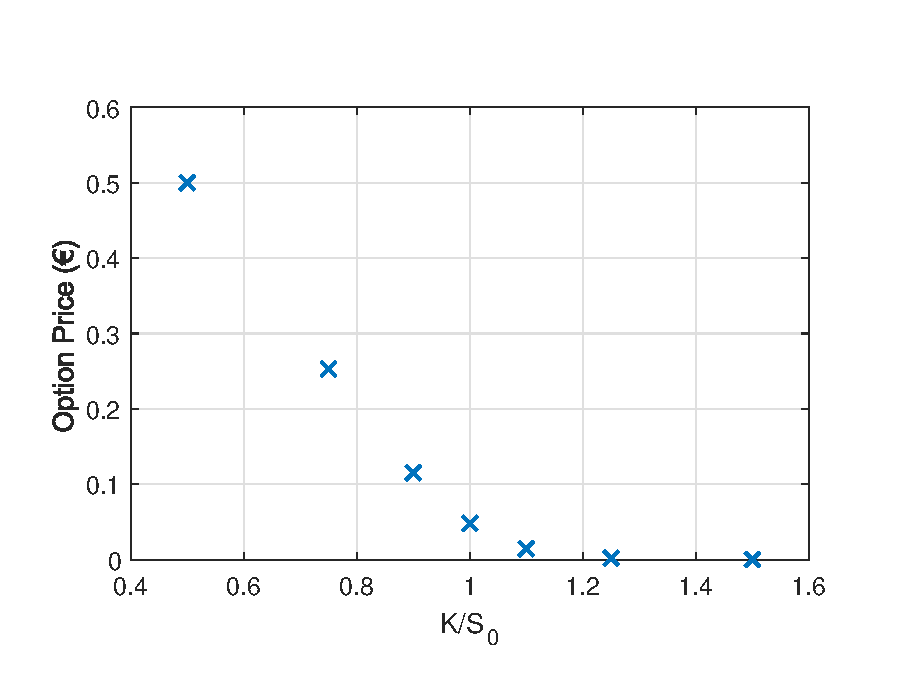
\includegraphics[width=0.47\linewidth,trim={0.25cm 0.45cm 1.1cm 1.4cm},clip]{T3P.eps}}
        \subfigure[Implied Volatility, T=126 days]{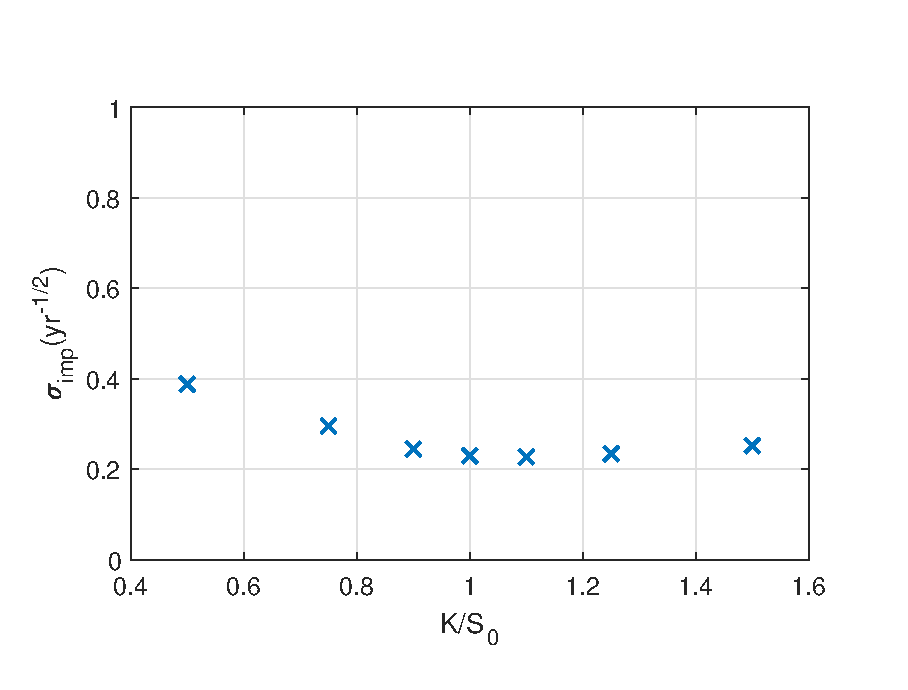
\includegraphics[width=0.47\linewidth,trim={0.25cm 0.45cm 1.1cm 1.4cm},clip]{T4.eps}}
    \subfigure[European Call Price, T=126 days]{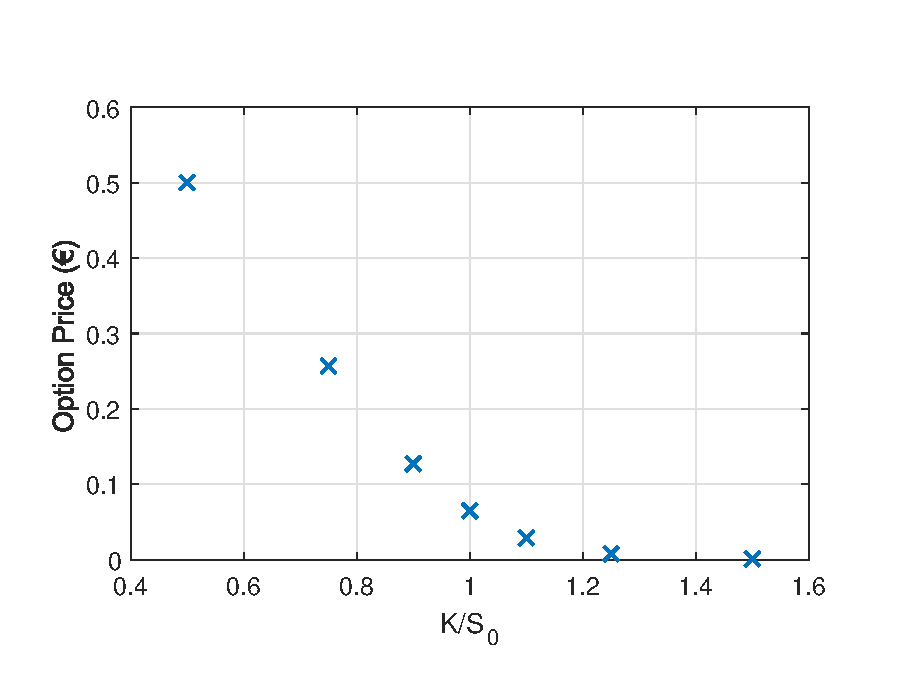
\includegraphics[width=0.47\linewidth,trim={0.25cm 0.45cm 1.1cm 1.4cm},clip]{T4P.eps}}
  \end{subfigmatrix}
  \caption[Scatter plots of the implied volatilities and European call prices provided]{Scatter plots of the implied volatilities and European call prices provided}
  \label{fig:mktdata}
\end{figure}


